\documentclass[12pt,fullpage,letterpaper]{article}

\newenvironment{proof}{\noindent{\bf Proof:}}{\qed\bigskip}

\newtheorem{theorem}{Theorem}
\newtheorem{corollary}{Corollary}
\newtheorem{lemma}{Lemma} 
\newtheorem{claim}{Claim}
\newtheorem{fact}{Fact}
\newtheorem{definition}{Definition}
\newtheorem{assumption}{Assumption}
\newtheorem{observation}{Observation}
\newtheorem{example}{Example}
\newcommand{\qed}{\rule{7pt}{7pt}}

\newcommand{\assignment}[4]{
\thispagestyle{plain} 
\newpage
\setcounter{page}{1}
\noindent
\begin{center}
\framebox{ \vbox{ \hbox to 6.28in
{\bf CS446: Machine Learning \hfill #1}
\vspace{4mm}
\hbox to 6.28in
{\hspace{2.5in}\large\mbox{Problem Set #2}}
\vspace{4mm}
\hbox to 6.28in
{{\it Handed Out: #3 \hfill Due: #4}}
}}
\end{center}
}


\newcommand{\handout}[3]{
\thispagestyle{plain} 
\newpage
\setcounter{page}{1}
\noindent
\begin{center}
\framebox{ \vbox{ \hbox to 6.28in
{\bf CS446: Machine Learning \hfill #1}
\vspace{4mm}
\hbox to 6.28in
{\hspace{2.5in}\large\mbox{#2}}
\vspace{4mm}
\hbox to 6.28in
{{\it Handed Out: #3 \hfill Name (NetID): \rule[-2pt]{4cm}{0.1pt} }}
}}
\end{center}
}


\newcommand{\assgsoln}[4]{
\thispagestyle{plain} 
\newpage
\setcounter{page}{1}
\noindent
\begin{center}
\framebox{ \vbox{ \hbox to 6.28in
{\bf CS446: Machine Learning \hfill #1}
\vspace{4mm}
\hbox to 6.28in
{\hspace{2.5in}\large\mbox{Problem Set #2 Solutions}}
\vspace{4mm}
\hbox to 6.28in
{{\it Handed Out: #3 \hfill Handed In: #4}}
}}
\end{center}
}


\newcommand{\solution}[4]{
\thispagestyle{plain} 
\newpage
\setcounter{page}{1}
\noindent
\begin{center}
\framebox{ \vbox{ \hbox to 6.28in
{\bf CS446: Machine Learning \hfill #4}
\vspace{4mm}
\hbox to 6.28in
{\hspace{2.5in}\large\mbox{Problem Set #3}}
\vspace{4mm}
\hbox to 6.28in
{#1 \hfill {\it Handed In: #2}}
}}
\end{center}
\markright{#1}
}


\newenvironment{algorithm}
{\begin{center}
\begin{tabular}{|l|}
\hline
\begin{minipage}{1in}
\begin{tabbing}
\quad\=\qquad\=\qquad\=\qquad\=\qquad\=\qquad\=\qquad\=\kill}
{\end{tabbing}
\end{minipage} \\
\hline
\end{tabular}
\end{center}}

\def\Comment#1{\textsf{\textsl{$\langle\!\langle$#1\/$\rangle\!\rangle$}}}


\usepackage{amsmath}
\usepackage{graphicx}
\usepackage{amsfonts}
\usepackage{amssymb}
\usepackage{array,multirow}
\usepackage{rotating}
\usepackage{graphicx}
\usepackage{caption}
\usepackage{subcaption}
\usepackage{threeparttable}
\newcommand{\bb}[1]{{\bf #1}}
\oddsidemargin 0in
\evensidemargin 0in
\textwidth 6.5in
\topmargin -0.5in
\textheight 9.0in

\begin{document}

\solution{Hsiang-Wei Hwang}{\today}{4}{Spring 2017}

\pagestyle{myheadings}  % Leave this command alone
\begin{enumerate}
\item{\textbf{[PAC Learning]}} 
	\begin{itemize}  
		\item[(a)]
The radii of the examples are the learning targets. If the example is positive, $r_2$ should be adjusted larger or equal to the radius of the example. On the other hand, if the example is negative, $r_1$ should be adjusted larger or equal to the radius of the example and $r_2$ should be larger or equal to $r_1$.\\
\textbf{An algorithm for learning: }\\ 
 \textit{Initialize: first positive example $x_1$, set $r_1 = |x_1|, r_2 = |x_1|$}\\
\textit{for all positive examples}\\
\hspace*{0cm} \textit{if $|x| > r_2$}\\
\hspace*{0.5cm} \textit{set $r_2 = |x|$}\\ 
\hspace*{0cm} \textit{if $|x| < r_1$}\\
\hspace*{0.5cm} \textit{set $r_1 = |x|$}\\ 
\item[(b)]
\begin{itemize}
\item[i.]
Only the examples satisfying  $r_1 \le |x| \le r_2$ are considered as positive by the classifier. Thus, the region out of learned function, $h_{r_1,r_2}$ but in target function, $h^*_{r_1^*,r_2^*}$, is the place misclassification happens which is $r_1^* \leq |x| \leq r_1$ or $r_2 < |x|_2 \leq r_2^*$.   
\item[ii.]
As mentioned, the fail rate of classification for one example is $\epsilon$. Thus, the probability that consistent with m examples is :
\begin{equation*}
	(1 - \epsilon)^m 
\end{equation*}
\end{itemize}
\item[(c)]
Assume the set $H_e$ is a subset of $H$ that any function $g$ in $H_e$ satisfies $Error(g) > \epsilon$. The probability that g is consistent with m examples is bounded by $(1 - \epsilon)^m $ which means that $P(g \in H_e\mbox{ consistent with m examples}) \le (1 - \epsilon)^m$. Thus, the probability we get h in $H_e$:
% \begin{equation*}
% 	\int \int_{\forall(r_2, r_1) \in M} 
% 	(\frac{ {r_2}^2 -  {r_1}^2} {  {r_2^*}^2 -  {r_1^*}^2})^m dr_2 dr_1 \le ({r_2^*} -  {r_1^*})^2(1 - \epsilon)^m < \delta
% \end{equation*}

\begin{equation*}
	P(|H_e|/|H|) * P(g \in H_e\mbox{ consistent with m examples}) \le 1 * (1 - \epsilon)^m <  \delta
\end{equation*}
\begin{equation*}
	\Rightarrow  e^{-\epsilon m} < \delta
	\Rightarrow - \epsilon m < \ln \delta 
	\Rightarrow m > \frac{1}{\epsilon}  \ln \frac{1}{\delta}
\end{equation*}
\item[(d)]
VC = 2 (Similar to VC(intervals)). According to the formula mentioned in the slide, 
\begin{equation*}
	 m > \frac{1}{\epsilon}\{ 8VC(H) \log \frac{13}{\epsilon} + 4\log \frac{2}{\delta} \}  
	\Rightarrow m > \frac{1}{\epsilon}\{ 16 \log \frac{13}{\epsilon} + 4\log \frac{2}{\delta} \} 
\end{equation*}




	\end{itemize}
	\clearpage
\item{\textbf{[VC Dimension]}} 
	\\We can adjust coefficients, a, b and c, to achieve any parabolic function required. Thus, 3-point case is achievable. \\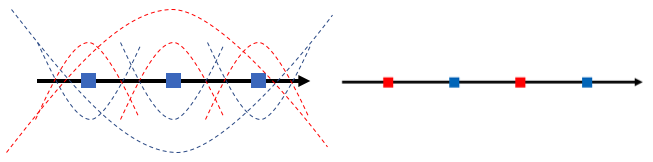
\includegraphics[width = 0.9\textwidth]{fig1.png}\\
According to the figure above, the 4-point case cannot be separated by parabolic functions. Thus, VC = 3.
\item{\textbf{[Kernels]}} 
	\begin{itemize}  
		\item[(a)]
According to the slide, $
\bf{w} = \sum_{(x_i,y_i) \in S} r\alpha_i x_iy_i,\mbox{ } y = sgn(\bf{w}^T x)
$ where r is the learning rate, $\alpha_i$ is the number of mistakes on the example, $(x_i,y_i)$. 
\item[(b)]
    Polynomial kernels functions, $K(\bb{x},\bb{x}')$, are defined as following description: \\
    1. Linear kernel: $K(\bb{x},\bb{x}') = \bb{x}\bb{x}'$. 2. Polynomial kernel of degree d: $K(\bb{x},\bb{x}') = (\bb{x}\bb{x}')^d$ (only dth-order interactions). 3. Polynomial kernel up to degree d: $K(\bb{x},\bb{x}') = (\bb{x}\bb{x}'+c)^d \ (c>0)$ (all interactions of order d or lower).\\ 
    Besides, kernel functions, $K(\bb{x},\bb{x}')$, can be constructed by few methods: 1. Multiply by a constant. 2. Multiply by a function f applied to \bb{x} and \bb{x'}. 3. Applying a polynomial (with non-negative coefficients) to $K(\bb{x},\bb{x}')$. 4. Exponentiating k(\bb{x}, \bb{x'}). 5. Add it and the other kernel function together. 6. Multiply by the other kernel function.\\
    According to the description of polynomial kernels, we get:
    \begin{equation*}
      K_1 = \vec{\bb{x}}^T\vec{\bb{z}}, K_2 = (\vec{\bb{x}}^T\vec{\bb{z}} + 4)^2, K_3 = (\vec{\bb{x}}^T\vec{\bb{z}})^3
    \end{equation*}
    According to the methods of constructing a kernel function, we can construct a kernel:    
    \begin{equation*}
      K' = K_3 + 49K_2 + 64K_1 = (\vec{\bb{x}}^T\vec{\bb{z}})^3 
                                      + 49(\vec{\bb{x}}^T\vec{\bb{z}} + 4)^2 
                                      + 64 \vec{\bb{x}}^T\vec{\bb{z}} = K'(\vec{\bb{x}},\vec{\bb{z}})
    \end{equation*}
    Thus, $K'(\vec{\bb{x}},\vec{\bb{z}})$ is a kernel.
\item[(c)]
\begin{equation*}
  K(\vec{x},\vec{z}) = 
  \begin{cases}
    {\vec{x}^T\vec{z} \choose k} & \mbox{if } \vec{x}^T\vec{z} \ge k \\
    0 & \mbox{otherwise}
  \end{cases}  
\end{equation*}
It represents the inner product of monotone conjunctions containing exactly k different variables. The inner product $\vec{x}^T\vec{z}$ means the number both variables are 1 in $\vec{x}$ and $\vec{z}$, and the monotone conjunctions containing exactly k different variables can be calculated by $\vec{x}^T\vec{z}$ choosing k that picking out k matches from the total matches to form a conjunction. For example, let k = 2, and $\vec{x}$ and $\vec{z}$ have 4 matches of 1, $\{x_2, x_5, x_6, x_8\}$ and $\{z_2, z_5, z_6, z_8\}$. We get a set that the monotone conjunctions are 1 in both vectors, $\{x_2x_5, x_2x_6, x_2x_8, x_5x_6, x_5x_8, x_6x_8 \}$ and $\{z_2z_5, z_2z_6, z_2z_8, z_5z_6, z_5z_8, z_6z_8 \}$, by combining all possible pairs. Thus, the number of the monotone conjunctions which inner product is 1 is 4 choose 2. 
This kernel can be computed in O(dm) that m means the number of the examples and d means the dimension of the vectors. Thus, this can be calculated in linear time.

	\end{itemize}
\item{\textbf{[SVM]}} 
	\begin{itemize}  
		\item[(a)]

\begin{itemize}
\item[1.]
Define $\mathbf{w}= (-1,-1)$, $\theta = 0$ 
\item[2.]
$\mathbf{w} = (-\frac{1}{2},-\frac{1}{2})$, $\theta = 0$ 
\item[3.]
We are finding a line that the distance from the point to the line represents the absolute value of $\vec{w}^T\vec{x}$ and the different side of the line represents the sign of $\vec{w}^T\vec{x}$. To maximize the margin, I consider the perpendicular bisectors of the closest pair of positive point and negative point, (-2,0) and (0,2). If I find the perpendicular bisector with distance to the points which is also the minimal distance of all points to this line, the line is the separator we are looking for.
\\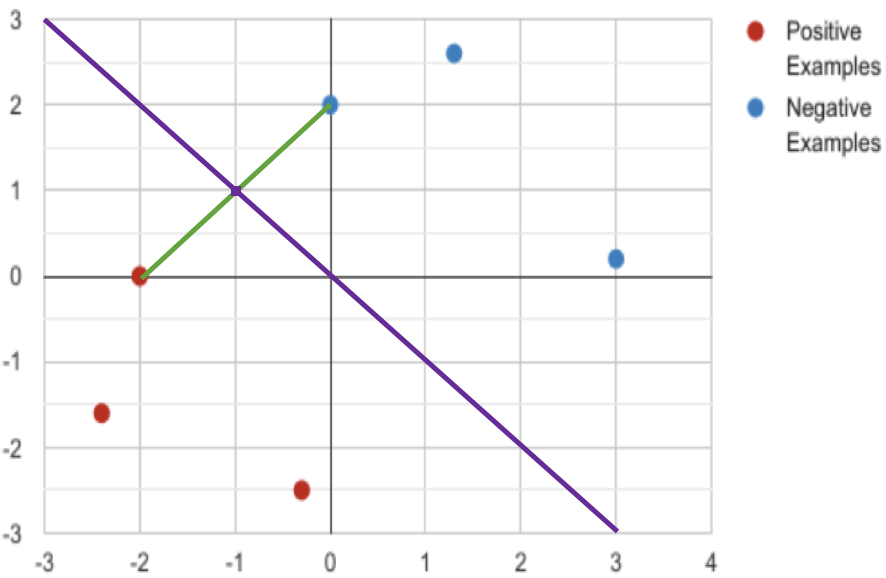
\includegraphics[width = 0.7\textwidth]{fig2.png}\\
\end{itemize}
\item[(b)]
\begin{itemize}
\item[1.]
As mentioned above, the support vectors are point 1 and point 6 which means I = \{1,6\}.
\item[2.]
 $\mathbf{w}^{*} = \sum \alpha_i y_i x_i \Rightarrow (-\frac{1}{2},-\frac{1}{2}) =\alpha_1\times 1 \times(-2,0)+\alpha_2\times -1\times(0,2) $.\\ Thus, $\{\alpha_1, \alpha_2\}=\{0.25,0.25\}$.  
\item[3.]
Objective function: $\frac{1}{2}||w||^2$ ($||w||$ calculated by L2 norm).\\
Objective function value $=\frac{1}{2}||w||^2 = \frac{1}{2} [(-0.5)^2+(-0.5)^2)] = 0.25 $.
\end{itemize} 
\item[(c)]
\textbf{For the case $C = 0$}, it shows that the algorithm will find the $w$ with the minimal absolute value without considering the loss. Thus, $\xi_i$ can be really big that the result can not separate the dataset anymore. More specifically, the algorithm will get $\bb{w} = \bb{0}$ and $\xi_{i} \ge 1$ which minimizing the objective function being zero, but representing nothing for separating the points. Thus, the smaller C we assign the better generalization we make, but C = 0 is too general that any dataset will satisfy the answer. \\
\textbf{For the case $C = \infty$}, the algorithm will try to make the term $\sum_{j=1}^{m}{\xi_{i}}$ zero because if there is anything nonzero in that term, the objective function value will blow up to $\infty$. Thus, all $\xi_{i}$ should be zero, and that makes the algorithm find $w$ with the most strict margin as \textbf{Hard SVM}. \textbf{The result would be the same as I have found in (a)-2.}\\
\textbf{For the case $C = 1$}, it is a balanced option between $C = 0$ and $C = \infty$. The algorithm will get us a $w$ between $w$ with the most strict margin and $w$ allowing any amount of loss. Thus, we will get a general and good solution for the dataset.

  
	\end{itemize}
\item{\textbf{[Boosting]}} 
	\begin{itemize}  
		\item[(a)(b)] \ \\
      \begin{tabular}{|c|c||c|c|c|c||c|c|c|c|}
        \hline
        & & \multicolumn{4}{c||}{Hypothesis 1} & \multicolumn{4}{c|}{Hypothesis 2} \\
        \cline{3-10}
        {\em i} & Label & $D_0$ & $f_1 \equiv $ & $f_2 \equiv $ & $h_1\equiv$ & $D_1$ &  $f_1 \equiv $ & $f_2 \equiv $ & $h_2 \equiv $ \\
        & & & [$x >$2$\;$] & [$y >$6$\;$] & [$x >$2$\;$] & & [$x >$9$\;$] & [$y >$11$\;$] & [$y >$11$\;$] \\

        \tiny{(1)} & \tiny{(2)} & \tiny{(3)} & \tiny{(4)} &  \tiny{(5)} & \tiny{(6)} & \tiny{(7)} & \tiny{(8)} & \tiny{(9)} & \tiny{(10)}\\
        \hline \hline
        {\em 1} & $-$ &0.1&$-$&$+$&$-$&$\frac{1}{16}$&$-$&$-$&$-$  \\
        \hline
        {\em 2} & $-$ &0.1&$-$&$-$&$-$&$\frac{1}{16}$&$-$&$-$&$-$  \\
        \hline
        {\em 3} & $+$ &0.1&$+$&$+$&$+$&$\frac{1}{16}$&$-$&$-$&$-$ \\
        \hline
        {\em 4} & $-$ &0.1&$-$&$-$&$-$&$\frac{1}{16}$&$-$&$-$&$-$ \\
        \hline
        {\em 5} & $-$ &0.1&$-$&$+$&$-$&$\frac{1}{16}$&$-$&$+$&$+$ \\
        \hline
        {\em 6} & $-$ &0.1&$+$&$+$&$+$&$\frac{1}{4}$&$-$&$-$&$-$ \\
        \hline
        {\em 7} & $+$ &0.1&$+$&$+$&$+$&$\frac{1}{16}$&$+$&$-$&$-$ \\
        \hline
        {\em 8} & $-$ &0.1&$-$&$-$&$-$&$\frac{1}{16}$&$-$&$-$&$-$ \\
        \hline
        {\em 9} & $+$ &0.1&$-$&$+$&$-$&$\frac{1}{4}$&$-$&$+$&$+$ \\
        \hline
        {\em 10} & $+$ &0.1&$+$&$+$&$+$&$\frac{1}{16}$&$-$&$-$&$-$ \\
        \hline
      \end{tabular}
\item[(c)]
\begin{equation*}
\epsilon_1 = \frac{2}{10}, \alpha_1 = \frac{1}{2} \ln{(1-\epsilon_1)/\epsilon_1} = \ln2, D_0 = \frac{1}{10},
\end{equation*}
\begin{equation*}
 z_0 = \sum D_0(i)\times exp(-\alpha_1 y_i h_0 (xi))= 0.1\times(2\times exp(\ln2)+8\times exp(-\ln2)) = 0.8
\end{equation*}
\begin{equation*}
D_1(i) = D_0(i)/z_0 \times  exp(-\alpha_1 y_i h_0 (xi)) =
  \begin{cases}
    0.1/0.8 \times 0.5 = \frac{1}{16} & \mbox{if } y_i h_0 (xi) = 1 \\
    0.1/0.8 \times 2 = \frac{1}{4} & \mbox{otherwise}
  \end{cases}   
\end{equation*}
\item[(d)]
\begin{equation*}
\epsilon_2 =  Pr_{D_1}[h_2(x_i) \lnot= y_i] =\frac{1}{16}\times4= \frac{1}{4}, \alpha_2 = \frac{1}{2} \ln{(1-\epsilon_2)/\epsilon_2} = \frac{1}{2}\ln3
\end{equation*}
Then, we combine $h_1$ and $h_2$ by $\alpha_i$:
\begin{equation*}
h_{final} =  \alpha_1h_1+\alpha_2h_2 = \ln2[x > 2] +\frac{1}{2}\ln3[y > 11]
\end{equation*}






	\end{itemize}

\end{enumerate}

\end{document}